\chapter{Théorie d'un réseau acoustique de résonateur de Helmholtz fini}
Le but du projet est de caractériser un réseau de résonateur de Helmholtz placés sur un guide d'onde. On dispose pour cela d'un banc de mesure représenté figure ~\ref{schema_infini}. Une simulation de la propagation dans le réseau pourra donc être confronté à une expérience.

\begin{figure}[!ht] \centering
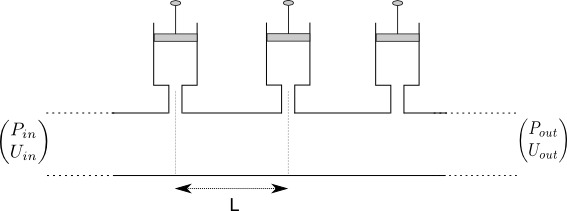
\includegraphics[scale=0.5]{./images_chp1/schema_reseau_infini.png}
\caption{\label{schema_infini} Schéma du réseau de résonateurs de Helmholtz.}
\end{figure}


\section{Mise sous forme matricielle}
On s’intéresse ici a la mise sous forme matricielle du problème de la propagation acoustique dans le réseau periodique vu ci-dessus. Le but étant de mettre le système sous la forme suivante:
\begin{equation}
\begin{pmatrix} P_{out} \\ U_{out} \end{pmatrix} =\begin{pmatrix} a & b \\ c & d \end{pmatrix}^N \begin{pmatrix} P_{in} \\ U_{in} \end{pmatrix} = \begin{pmatrix} A & B \\ C & D \end{pmatrix} \begin{pmatrix} P_{in} \\ U_{in} \end{pmatrix} 
\end{equation}

Cette matrice dispose en effet de propriétés intéressantes et l'étude du système sera grandement facilité par ce formalise. De plus, les simulations sont faciles à mettre en œuvre dès lors que celle ci est connue.

Pour cela, les 2 éléments du réseau (guide et résonateur) doivent être mis sous forme matricielle puis multipliés.

\subsection{Le guide d'onde}
La solution de la propagation dans un guide d'onde peux être facilement déduite de l'équation d'onde suivante:
\begin{equation}
\frac{\partial ^2 p}{\partial x^2} -\frac{1}{c^{2}} \frac{\partial ^2 p}{\partial t^2}= 0
\end{equation}

On se place en régime harmonique et on note $\Gamma = jk$ la constante de propagation du système. D’où les solutions (vitesses calculées avec l'équation d'Euler:

\begin{eqnarray*}
\begin{cases}
p(x_1)  =  C1 e^{-\Gamma x_1} + C2 e^{\Gamma x_1} \\
v(x_1)  =  -\frac{1}{j\omega\rho} [ -\Gamma C1 e^{-\Gamma x_1} + \Gamma e^{\Gamma x_1}]\\
p(x_2)  =  C1 e^{-\Gamma x_2} + C2 e^{\Gamma x_2} \\
v(x_2)  =  -\frac{1}{j\omega\rho} [ -\Gamma C1 e^{-\Gamma x_2} + \Gamma e^{\Gamma x_2}]
\end{cases}
\end{eqnarray*}
 
On pose $x_1 - x_2 = L$. Tous calculs faits, on trouve finalement:
\begin{eqnarray*}
\begin{pmatrix} p(x_1) \\ v(x_1) \end{pmatrix} = \begin{pmatrix} \cosh(kL) & \frac{j\omega\rho}{k} \sinh(k L) \\  \frac{k}{j\omega\rho}\sinh(k L) & \cosh(k L) \end{pmatrix} \begin{pmatrix} p(x_2) \\ v(x_2) \end{pmatrix}
\end{eqnarray*}

La première fréquence de coupure du guide est donc d'environ $4kHz$ pour les dimensions du réseau que nous considérons. Dans la suite, on supposera donc que seul le mode plan est propagatif. Les simulations et mesures ne seront donc faite que sur une bande de fréquences allant de $0$ à $1~kHz$.

\subsubsection{Ajout des pertes}

Pour prendre en compte les pertes, on modifie l'expression de la constante de propagation et de l'impédance caractéristique. Les expressions sont donc:
\begin{eqnarray*}
 k =  \frac{\omega}{c_0} \left( 1 + \frac{\beta}{s}(1+(\gamma-1)/ \chi \right) \\
 Z_c =  \frac{\rho c_0}{S} \left( 1 + \frac{\beta}{s}(1-(\gamma-1)/ \chi \right) 
\end{eqnarray*}

Dans ces expressions, on a:
\begin{itemize}
 \item  $s=R/ \delta$ avec $\delta = \sqrt{\frac{2 \mu}{\rho \omega}}$
 \item  $\chi = \sqrt{P_r}$ ou $P_r$ est le nombre de Prandtl
 \item $\beta = (1-j)/\sqrt{2}$ 
 \item $\mu$ la viscosité de l'air
\end{itemize}

Du fait de la géométrie assez complexe du système, ces pertes ne peuvent pas être négligées comme cela peux être souvent le cas en acoustique.

\subsection{Le résonateur}
Le résonateur de Helmholtz est considéré dans le réseau comme un changement ponctuel d'impédance. Cette impédance peux etre calculée via la formule de l'impédance ramenée ~\ref{imp_ramenee}. De plus, les dimensions utilisées dans la suite sont corrigées afin de prendre en compte les corrections de longueurs liés à la géométrie du problèmes. Ces formules de corrections sont disponibles en annexe 2.
\begin{eqnarray}
Z{x_1}=\frac{jZ_c tan(kL)+Z_{x_2}}{1+j\frac{Z_{x_2}}{Z_c}tan(kL)}.
%\label{imp_ramenee}
\end{eqnarray}

Si on suppose que le résonateur est constitué d'une parois rigide et de 2 tubes, on peux calculer sont impédance comme suit:

\begin{eqnarray*}
\begin{pmatrix} P_2 \\U_2 \end{pmatrix} & = & \begin{pmatrix} \cos(k l) & j Z_{c_1} \sin(k l) \\ \frac{1}{Z_{c_1}} \sin(k l) & \cos(k l) \end{pmatrix} \begin{pmatrix} \cos(k L) & j Z_{c_2} \sin(k L) \\ \frac{1}{Z_{c_2}} \sin(k L) & \cos(k L) \end{pmatrix} \begin{pmatrix} P_1 \\ 0  \end{pmatrix} \\
\begin{pmatrix} P_2 \\U_2 \end{pmatrix} & = & \begin{pmatrix} r_1 & r_2 \\ r_3 & r_4 \end{pmatrix} \begin{pmatrix} P_1 \\ 0  \end{pmatrix} \\
~ & \Leftrightarrow & Z_{resonateur} = \frac{A}{C}
\end{eqnarray*}

Si on ajoute un résonateur en parallèle au guide, on a toujours continuité des pressions mais plus des vitesses. On a donc la matrice de transfert pression-vitesse suivante pour un résonateur dans le réseau:

\begin{eqnarray*}
M_{resonateur} = \begin{pmatrix} 1 &  0 \\ 1 /Z_{resonateur} & 1  \end{pmatrix}\\
\end{eqnarray*}

\section{Étude du réseau fini}

Une fois les matrices de guide et de résonateur connues, il suffit alors de les multiplier afin d'obtenir la matrice d'une cellule du réseau. C'est sur l'étude de cette matrice que ce base les analyses de cette section. 

Dans la suite les paramètres de la simulation sont ceux du de l'expérience dont nous disposons. Ces paramètres sont disponible en annexe 2.

\subsection{Équation de dispersion}
On peux déduire de la matrice de transfert l'équation de dispersion pour le réseau à N cellules, on a en effet:
\begin{equation}
\cos(NkL) = \frac{A+D}{2} 
\end{equation}

Ainsi, on peux remonter à une expression de $kL$ en fonction de la fréquence. En particulier, les zones ou $kL$ devient imaginaire nous intéresse particulièrement car cela induit une décroissance exponentielle de l'onde de propageant dans le guilde. Ces bandes sont visible sur la figure ~\ref{bande_bragg} et sont appelées les bandes de Bragg.

\todo{une figure de l’équation de dispersion avec bande de bragg}

\subsection{Bande de Bragg}
Ces bandes de Bragg apparaissant dès qu'un élément est présent dans un réseau et ce de manière periodique. L'énergie de l'onde reste "enfermée" entre chaque éléments du fait que la longueur d'onde correspond à la moitié de l'espacement entre 2 éléments.  \todo{vérifier ça}.
 

\subsection{Bande interdites liés aux résonateurs}
L'équation de dispersion est cependant plus difficile analyser qu'il n'y parait du faite que ce sont des résonateurs qui servent d’éléments au réseau. Hors ce ci ont une impédance négligeable dès lors que la fréquence d'analyse ce trouve suffisamment éloignées des fréquences de résonances. 

De plus le résonateur étant par nature un système résonant, il peux lui aussi induire une absorption de l'énergie de l'onde sur certaines fréquences.

Il y a donc 2 phénomènes qui peuvent induire des bandes interdites, d'une part les bandes de Bragg liés a la géométrie du réseau et d'autre part l'énergie absorbée par les résonateurs.
\todo{Double figure explicative avec les 2 types de bande}.


\subsection{Réflexion et transmission du réseau}
On peux enfin tracer le coefficient de réflexion et de transmission du réseau complet. En effet, on a:
\begin{eqnarray}
T & = & \frac{2}{A + B/Z_c + C Z_c + D} \\
R & = & \frac{A + B / Zc_ - C Z_c -D}{A + B/Z_c + C Z_c + D} 
\end{eqnarray}

On obtient des résultats de ce type:
\todo{figure de Réflexion et transmission type}
